% Chapter 3: Word2Vec and Vector Operations

\section{Word2Vec}

% Word2Vec Training
\begin{frame}{Learning Embeddings: Word2Vec}
\textbf{How Do We Learn These Vectors?}

\begin{columns}
\column{0.5\textwidth}
\textbf{The Distributional Hypothesis:}
\begin{center}
\colorbox{yellow!20}{\parbox{0.9\columnwidth}{
``You shall know a word by the company it keeps'' - Firth (1957)
}}
\end{center}

\textbf{Two Approaches:}

\textbf{1. Skip-gram:} Predict context from word
\begin{center}
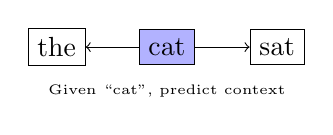
\begin{tikzpicture}[scale=0.7]
    \node[draw, fill=blue!30] (center) at (0,0) {cat};
    \node[draw] (w1) at (-2,0) {the};
    \node[draw] (w2) at (2,0) {sat};
    
    \draw[->] (center) -- (w1);
    \draw[->] (center) -- (w2);
    
    \node at (0,-0.8) {\tiny Given ``cat'', predict context};
\end{tikzpicture}
\end{center}

\textbf{2. CBOW:} Predict word from context
\begin{center}
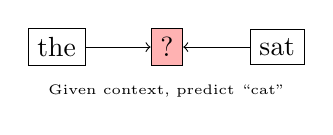
\begin{tikzpicture}[scale=0.7]
    \node[draw] (w1) at (-2,0) {the};
    \node[draw] (w2) at (2,0) {sat};
    \node[draw, fill=red!30] (center) at (0,0) {?};
    
    \draw[->] (w1) -- (center);
    \draw[->] (w2) -- (center);
    
    \node at (0,-0.8) {\tiny Given context, predict ``cat''};
\end{tikzpicture}
\end{center}

\column{0.5\textwidth}
\textbf{Training Process Visualization:}
\begin{center}
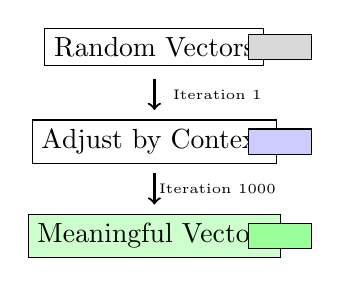
\begin{tikzpicture}[scale=0.8]
    % Initial random
    \node[draw] (init) at (0,3) {Random Vectors};
    \draw[fill=gray!30] (1.5,2.8) rectangle (2.5,3.2);
    
    % Training iterations
    \draw[->, thick] (0,2.5) -- (0,2);
    \node at (1,2.25) {\tiny Iteration 1};
    
    \node[draw] (iter1) at (0,1.5) {Adjust by Context};
    \draw[fill=blue!20] (1.5,1.3) rectangle (2.5,1.7);
    
    \draw[->, thick] (0,1) -- (0,0.5);
    \node at (1,0.75) {\tiny Iteration 1000};
    
    \node[draw, fill=green!20] (final) at (0,0) {Meaningful Vectors};
    \draw[fill=green!40] (1.5,-0.2) rectangle (2.5,0.2);
\end{tikzpicture}
\end{center}

\textbf{Objective Function:}
$$\max \sum_{t=1}^{T} \sum_{-c \leq j \leq c} \log P(w_{t+j} | w_t)$$

Maximize probability of context words
\end{columns}
\end{frame}

% Vector Arithmetic
\begin{frame}{Vector Arithmetic: The Surprising Discovery}
\textbf{Embeddings Capture Analogies!}

\begin{columns}
\column{0.5\textwidth}
\textbf{Famous Examples:}

\begin{center}
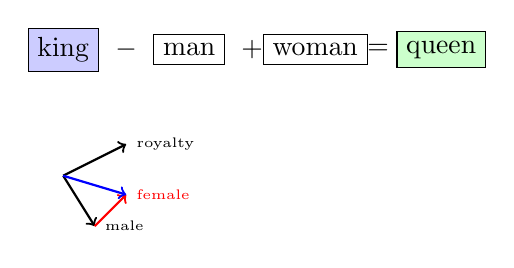
\begin{tikzpicture}[scale=0.8]
    % King - Man + Woman = Queen
    \node[draw, fill=blue!20] (king) at (0,2) {king};
    \node[draw] (man) at (2,2) {man};
    \node[draw] (woman) at (4,2) {woman};
    \node[draw, fill=green!20] (queen) at (6,2) {queen};
    
    \node at (1,2) {$-$};
    \node at (3,2) {$+$};
    \node at (5,2) {$=$};
    
    % Vector visualization
    \draw[->, thick] (0,0) -- (1,0.5) node[right] {\tiny royalty};
    \draw[->, thick] (0,0) -- (0.5,-0.8) node[right] {\tiny male};
    \draw[->, thick, red] (0.5,-0.8) -- (1,-0.3) node[right] {\tiny female};
    \draw[->, thick, blue] (0,0) -- (1,-0.3);
\end{tikzpicture}
\end{center}

\textbf{More Analogies:}
\begin{itemize}
    \item Paris - France + Germany = Berlin
    \item bigger - big + small = smaller
    \item walked - walk + run = ran
\end{itemize}

\column{0.5\textwidth}
\textbf{Why Does This Work?}

\begin{center}
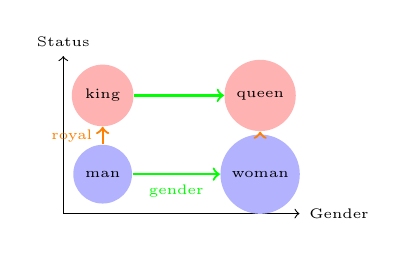
\begin{tikzpicture}[scale=1]
    % Draw coordinate system
    \draw[->] (0,0) -- (3,0) node[right] {\tiny Gender};
    \draw[->] (0,0) -- (0,2) node[above] {\tiny Status};
    
    % Plot words
    \node[circle, fill=blue!30] (man) at (0.5,0.5) {\tiny man};
    \node[circle, fill=blue!30] (woman) at (2.5,0.5) {\tiny woman};
    \node[circle, fill=red!30] (king) at (0.5,1.5) {\tiny king};
    \node[circle, fill=red!30] (queen) at (2.5,1.5) {\tiny queen};
    
    % Show relationships
    \draw[->, thick, green] (man) -- (woman) node[midway, below] {\tiny gender};
    \draw[->, thick, green] (king) -- (queen);
    
    \draw[->, thick, orange] (man) -- (king) node[midway, left] {\tiny royal};
    \draw[->, thick, orange] (woman) -- (queen);
\end{tikzpicture}
\end{center}

\textbf{The Pattern:}
\begin{itemize}
    \item Relationships are \textbf{directions}
    \item Same relationship = same direction
    \item Linear structure emerges naturally!
\end{itemize}
\end{columns}

\vspace{0.2cm}
\begin{center}
\colorbox{green!10}{\parbox{0.9\textwidth}{
\textbf{Remarkable:} These patterns were never explicitly programmed - they emerge from the data!
}}
\end{center}
\end{frame}

% Measuring Similarity
\begin{frame}{Measuring Word Similarity}
\textbf{How Similar Are Two Words?}

\begin{columns}
\column{0.5\textwidth}
\textbf{Cosine Similarity:}
$$\text{similarity}(A, B) = \frac{A \cdot B}{||A|| \times ||B||} = \cos(\theta)$$

\begin{center}
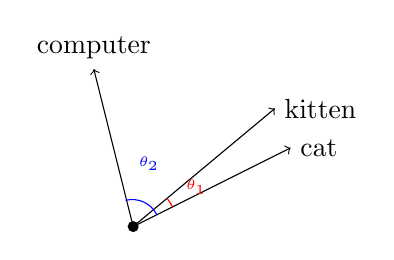
\begin{tikzpicture}[scale=1]
    % Draw vectors
    \draw[->] (0,0) -- (2,1) node[right] {cat};
    \draw[->] (0,0) -- (1.8,1.5) node[right] {kitten};
    \draw[->] (0,0) -- (-0.5,2) node[above] {computer};
    
    % Show angle
    \draw[red] (0.5,0.25) arc (26.57:40:0.56);
    \node[red] at (0.8,0.5) {\tiny $\theta_1$};
    
    \draw[blue] (0.3,0.15) arc (26.57:104:0.35);
    \node[blue] at (0.2,0.8) {\tiny $\theta_2$};
    
    % Origin
    \fill (0,0) circle (2pt);
\end{tikzpicture}
\end{center}

\begin{itemize}
    \item cat $\sim$ kitten: $\cos(\theta_1) = 0.95$
    \item cat $\sim$ computer: $\cos(\theta_2) = 0.1$
\end{itemize}

\column{0.5\textwidth}
\textbf{Similarity Matrix Example:}
\begin{center}
\footnotesize
\begin{tabular}{|c|c|c|c|c|}
\hline
 & cat & dog & car & truck \\
\hline
cat & 1.0 & 0.8 & 0.1 & 0.05 \\
\hline
dog & 0.8 & 1.0 & 0.15 & 0.1 \\
\hline
car & 0.1 & 0.15 & 1.0 & 0.85 \\
\hline
truck & 0.05 & 0.1 & 0.85 & 1.0 \\
\hline
\end{tabular}
\end{center}

\textbf{Visual Heatmap:}
\begin{center}
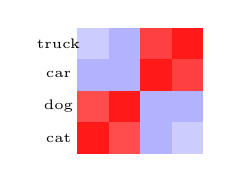
\begin{tikzpicture}[scale=0.8]
    % Draw heatmap
    \fill[red!90] (0,0) rectangle (0.5,0.5);
    \fill[red!70] (0.5,0) rectangle (1,0.5);
    \fill[blue!30] (1,0) rectangle (1.5,0.5);
    \fill[blue!20] (1.5,0) rectangle (2,0.5);
    
    \fill[red!70] (0,0.5) rectangle (0.5,1);
    \fill[red!90] (0.5,0.5) rectangle (1,1);
    \fill[blue!30] (1,0.5) rectangle (1.5,1);
    \fill[blue!30] (1.5,0.5) rectangle (2,1);
    
    \fill[blue!30] (0,1) rectangle (0.5,1.5);
    \fill[blue!30] (0.5,1) rectangle (1,1.5);
    \fill[red!90] (1,1) rectangle (1.5,1.5);
    \fill[red!75] (1.5,1) rectangle (2,1.5);
    
    \fill[blue!20] (0,1.5) rectangle (0.5,2);
    \fill[blue!30] (0.5,1.5) rectangle (1,2);
    \fill[red!75] (1,1.5) rectangle (1.5,2);
    \fill[red!90] (1.5,1.5) rectangle (2,2);
    
    \node at (-0.3,0.25) {\tiny cat};
    \node at (-0.3,0.75) {\tiny dog};
    \node at (-0.3,1.25) {\tiny car};
    \node at (-0.3,1.75) {\tiny truck};
\end{tikzpicture}
\end{center}

Animals cluster together, vehicles cluster together!
\end{columns}
\end{frame}